\documentclass[11pt]{amsart}
\usepackage[letterpaper,margin=1in]{geometry}
\usepackage{amssymb}
\usepackage{tikz}
\usepackage[font=small,labelfont=bf]{caption}
\usepackage[hidelinks]{hyperref}
\newif\ifreview
\reviewfalse % \reviewfalse for the public preprint (no line numbers)
\ifreview\usepackage[switch]{lineno}\linenumbers\fi % JoCG review copies need line numbers
\hypersetup{pdftitle={Two Triangulations That Share Only Their Hull},pdfauthor={Vamshi Jandhyala}}

\definecolor{layerA}{RGB}{34,88,156}
\definecolor{layerB}{RGB}{174,53,40}
\tikzset{hull/.style={draw=black,line width=1.5pt},
 vertex/.style={circle,fill=black,inner sep=1.3pt},
 every picture/.style={line join=round,line cap=round}}

\newtheorem{theorem}{Theorem}
\newtheorem{lemma}[theorem]{Lemma}
\newtheorem{corollary}[theorem]{Corollary}
\theoremstyle{definition}
\newtheorem{definition}[theorem]{Definition}
\newcommand{\inter}{\operatorname{int}}

\newif\ifanon
\anonfalse % \anonfalse for the named version

\title{Two Triangulations That Share Only Their Hull}
\ifanon\else
\author{Vamshi Jandhyala}
\address{London, United Kingdom}
\email{vamshi.jandhyala@gmail.com}
\fi
\subjclass[2020]{52C45, 05C10, 05C62}
\keywords{Triangulations, point sets, geometric thickness, order types}
\date{7 October 2026}

\begin{document}

\begin{abstract}
Any two triangulations of a finite planar point set share the edges of its convex hull. We show that for every $n\geq9$ there are $n$ points in general position, with a pentagonal hull, that have two triangulations sharing nothing else. At least five edges must be shared whenever $n\geq5$, so this settles the minimum. The construction starts from nine explicit points and inserts points one at a time, carrying along a configuration that makes the next insertion possible. Started from a convex polygon, the same construction settles every hull size: $n$ points with $h$ hull vertices admit two triangulations sharing only the hull exactly when $n=h$, or $h\geq6$, or $h=5$ and $n\geq9$. The impossible cases with a pentagonal hull and six to eight points rest on an exhaustive search over order types, which also gives the minimum $4,5,6,6,6,5,5$ for $n=4,\dots,10$.
\end{abstract}

\maketitle

\section{Introduction}

How few edges can two triangulations of the same planar point set have in common? The hull edges are forced, but it is not apparent whether anything else must be shared once points lie inside the hull.

Let $P$ be a set of $n$ points in the plane, no three on a line. A \emph{triangulation} of $P$ is a maximal set of pairwise non-crossing segments with endpoints in $P$; it divides the convex hull of $P$ into triangles, its \emph{faces}. No edge can cross an edge of the convex hull, so every triangulation contains every hull edge, and two triangulations of $P$ always share at least as many edges as the hull has vertices.

Five points in convex position give a first answer. Number them $1$ to $5$ around the pentagon. The triangulation with diagonals $13$ and $14$ and the one with diagonals $24$ and $25$ have no diagonal in common, so they share only the five hull edges. Now put a sixth point inside the pentagon and try to keep this property. A search over all small point sets (Section~\ref{sec:small}) shows that it cannot be done with six, seven or eight points. With nine it can (Figure~\ref{fig:nine}).

\begin{figure}[t]
\centering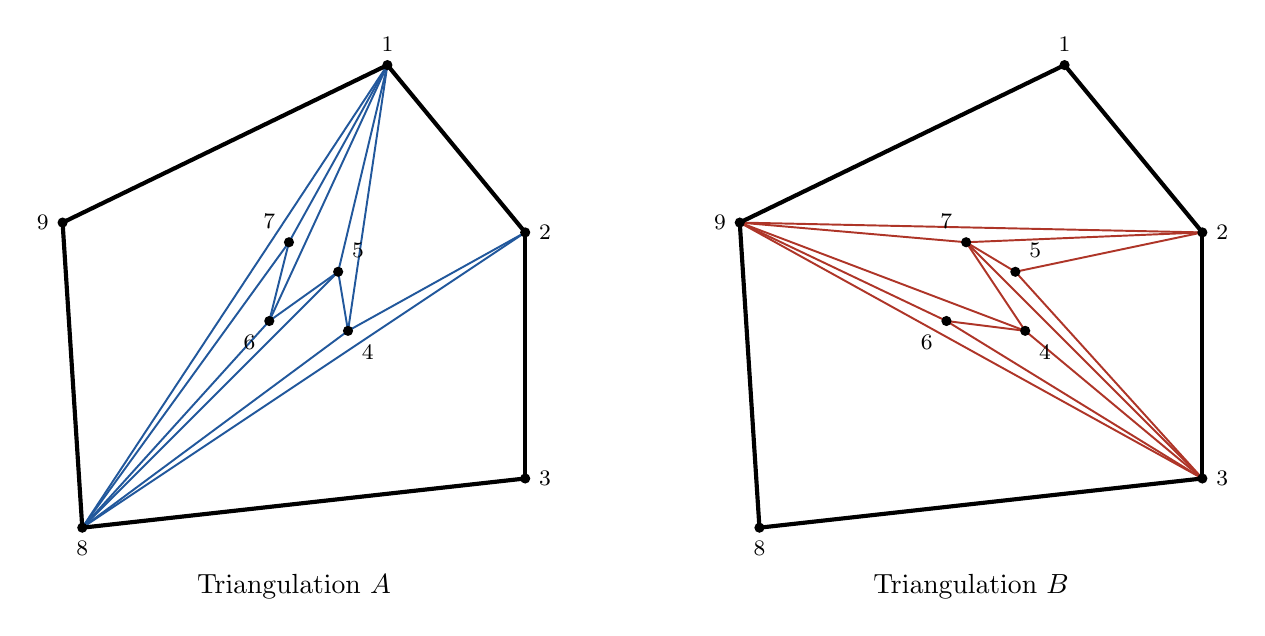
\begin{tikzpicture}[]
\draw[draw=layerA,line width=.7pt] (4.125,5.875) -- (3.625,2.500);
\draw[draw=layerA,line width=.7pt] (4.125,5.875) -- (3.500,3.250);
\draw[draw=layerA,line width=.7pt] (4.125,5.875) -- (2.625,2.625);
\draw[draw=layerA,line width=.7pt] (4.125,5.875) -- (2.875,3.625);
\draw[draw=layerA,line width=.7pt] (4.125,5.875) -- (0.250,0.000);
\draw[draw=layerA,line width=.7pt] (5.875,3.750) -- (3.625,2.500);
\draw[draw=layerA,line width=.7pt] (5.875,3.750) -- (0.250,0.000);
\draw[draw=layerA,line width=.7pt] (3.625,2.500) -- (3.500,3.250);
\draw[draw=layerA,line width=.7pt] (3.625,2.500) -- (0.250,0.000);
\draw[draw=layerA,line width=.7pt] (3.500,3.250) -- (2.625,2.625);
\draw[draw=layerA,line width=.7pt] (3.500,3.250) -- (0.250,0.000);
\draw[draw=layerA,line width=.7pt] (2.625,2.625) -- (2.875,3.625);
\draw[draw=layerA,line width=.7pt] (2.625,2.625) -- (0.250,0.000);
\draw[draw=layerA,line width=.7pt] (2.875,3.625) -- (0.250,0.000);
\draw[hull] (4.125,5.875) -- (5.875,3.750);
\draw[hull] (4.125,5.875) -- (0.000,3.875);
\draw[hull] (5.875,3.750) -- (5.875,0.625);
\draw[hull] (5.875,0.625) -- (0.250,0.000);
\draw[hull] (0.250,0.000) -- (0.000,3.875);
\node[vertex] at (4.125,5.875) {};
\node[above=1.5pt,font=\footnotesize] at (4.125,5.875) {$1$};
\node[vertex] at (5.875,3.750) {};
\node[right=1.5pt,font=\footnotesize] at (5.875,3.750) {$2$};
\node[vertex] at (5.875,0.625) {};
\node[right=1.5pt,font=\footnotesize] at (5.875,0.625) {$3$};
\node[vertex] at (3.625,2.500) {};
\node[below right=1.5pt,font=\footnotesize] at (3.625,2.500) {$4$};
\node[vertex] at (3.500,3.250) {};
\node[above right=1.5pt,font=\footnotesize] at (3.500,3.250) {$5$};
\node[vertex] at (2.625,2.625) {};
\node[below left=1.5pt,font=\footnotesize] at (2.625,2.625) {$6$};
\node[vertex] at (2.875,3.625) {};
\node[above left=1.5pt,font=\footnotesize] at (2.875,3.625) {$7$};
\node[vertex] at (0.250,0.000) {};
\node[below=1.5pt,font=\footnotesize] at (0.250,0.000) {$8$};
\node[vertex] at (0.000,3.875) {};
\node[left=1.5pt,font=\footnotesize] at (0.000,3.875) {$9$};
\node at (2.938,-0.75) {Triangulation $A$};
\draw[draw=layerB,line width=.7pt] (14.475,3.750) -- (12.100,3.250);
\draw[draw=layerB,line width=.7pt] (14.475,3.750) -- (11.475,3.625);
\draw[draw=layerB,line width=.7pt] (14.475,3.750) -- (8.600,3.875);
\draw[draw=layerB,line width=.7pt] (14.475,0.625) -- (12.225,2.500);
\draw[draw=layerB,line width=.7pt] (14.475,0.625) -- (12.100,3.250);
\draw[draw=layerB,line width=.7pt] (14.475,0.625) -- (11.225,2.625);
\draw[draw=layerB,line width=.7pt] (14.475,0.625) -- (11.475,3.625);
\draw[draw=layerB,line width=.7pt] (14.475,0.625) -- (8.600,3.875);
\draw[draw=layerB,line width=.7pt] (12.225,2.500) -- (11.225,2.625);
\draw[draw=layerB,line width=.7pt] (12.225,2.500) -- (11.475,3.625);
\draw[draw=layerB,line width=.7pt] (12.225,2.500) -- (8.600,3.875);
\draw[draw=layerB,line width=.7pt] (12.100,3.250) -- (11.475,3.625);
\draw[draw=layerB,line width=.7pt] (11.225,2.625) -- (8.600,3.875);
\draw[draw=layerB,line width=.7pt] (11.475,3.625) -- (8.600,3.875);
\draw[hull] (12.725,5.875) -- (14.475,3.750);
\draw[hull] (12.725,5.875) -- (8.600,3.875);
\draw[hull] (14.475,3.750) -- (14.475,0.625);
\draw[hull] (14.475,0.625) -- (8.850,0.000);
\draw[hull] (8.850,0.000) -- (8.600,3.875);
\node[vertex] at (12.725,5.875) {};
\node[above=1.5pt,font=\footnotesize] at (12.725,5.875) {$1$};
\node[vertex] at (14.475,3.750) {};
\node[right=1.5pt,font=\footnotesize] at (14.475,3.750) {$2$};
\node[vertex] at (14.475,0.625) {};
\node[right=1.5pt,font=\footnotesize] at (14.475,0.625) {$3$};
\node[vertex] at (12.225,2.500) {};
\node[below right=1.5pt,font=\footnotesize] at (12.225,2.500) {$4$};
\node[vertex] at (12.100,3.250) {};
\node[above right=1.5pt,font=\footnotesize] at (12.100,3.250) {$5$};
\node[vertex] at (11.225,2.625) {};
\node[below left=1.5pt,font=\footnotesize] at (11.225,2.625) {$6$};
\node[vertex] at (11.475,3.625) {};
\node[above left=1.5pt,font=\footnotesize] at (11.475,3.625) {$7$};
\node[vertex] at (8.850,0.000) {};
\node[below=1.5pt,font=\footnotesize] at (8.850,0.000) {$8$};
\node[vertex] at (8.600,3.875) {};
\node[left=1.5pt,font=\footnotesize] at (8.600,3.875) {$9$};
\node at (11.537,-0.75) {Triangulation $B$};
\end{tikzpicture}

\caption{Two triangulations of nine points whose only common edges are the five hull edges (black).}\label{fig:nine}
\end{figure}

The question was raised on MathOverflow in 2023~\cite{MO}. Write
\[
f(n)=\min_{|P|=n}\ \min_{A,B}\ |A\cap B|,
\]
where $P$ ranges over sets of $n$ points in general position and $A,B$ over triangulations of $P$, each regarded as a set of edges. Contributors to the thread observed that a triangular or quadrilateral hull with an interior point forces at least six shared edges, so that $f(n)\geq5$ for $n\geq5$ and five can only occur with a pentagonal hull; this also follows from the forced-edge argument of~\cite{HSV}. Random searches found pairs sharing six edges for $8\leq n\leq11$, but none sharing five.

\begin{theorem}\label{thm:main}
For every $n\geq9$ there is a set of $n$ points in general position with a pentagonal hull and two triangulations whose only common edges are the five hull edges. Hence $f(n)=5$ for all $n\geq9$.
\end{theorem}

The author posted Theorem~\ref{thm:main}, with the nine-point example and the insertion argument, as an answer to that question on 30 September 2026~\cite{MOAnswer}. Theorem~\ref{thm:hull} below is new here.

The question is related to geometric thickness. A graph is \emph{doubly linear} if it can be drawn with straight edges on some point set so that its edges split into two non-crossing classes; Hutchinson, Shermer, and Vince~\cite{HSV} showed that such a graph on $n\geq4$ vertices has at most $6n-18$ edges. For a point set with a triangular hull, each triangulation has $3n-6$ edges, so two triangulations sharing $s$ edges have a union of $6n-12-s$ edges: the shared ones would otherwise be counted twice. The union splits into two non-crossing classes, so the bound says $s\geq6$ there, and equality would require a doubly linear graph with $6n-18$ edges. Durocher, Gethner, and Mondal~\cite{DGM} constructed doubly linear graphs with $6n-19$ edges for every $n\geq9$, and completing their two layers to triangulations shows $f(n)\leq7$. Theorem~\ref{thm:main} does not bear on whether $6n-18$ edges are possible. That question needs a triangular hull, and with a pentagonal hull the union of the two triangulations has only $2(3n-8)-5=6n-21$ edges.

The question also makes sense for each hull size separately. Garc\'{\i}a, Hurtado, Korman, Matos, Saumell, Silveira, Tejel, and T\'oth~\cite{GHK} studied \emph{biplane} graphs on a fixed point set, those whose edges split into two non-crossing classes. A maximal biplane graph on $P$ is the union of two triangulations~\cite[Lemma~1]{GHK}, so if the hull of $P$ has $h$ vertices it has at most $2(3n-3-h)-h=6n-3h-6$ edges, with equality exactly when the two triangulations share only the hull. For the nine points of Figure~\ref{fig:nine}, with $h=5$, each triangulation has $3\cdot9-3-5=19$ edges and their union has $2\cdot19-5=33=6\cdot9-3\cdot5-6$. The second theorem says when that happens.

\begin{theorem}\label{thm:hull}
Let $3\leq h\leq n$. There is a set of $n$ points in general position with $h$ hull vertices and two triangulations whose only common edges are the $h$ hull edges if and only if $n=h$, or $h\geq6$, or $h=5$ and $n\geq9$.
\end{theorem}

The nonexistence assertion for a pentagonal hull with six to eight points is computer-assisted (Section~\ref{sec:small}); all other cases have geometric proofs. A triangular or quadrilateral hull with a point inside always forces extra shared edges. For every $h\geq6$ and $n\geq h$, some point set attains hull-only sharing. The pentagon of the opening example is the only hull size with a gap.

Section~\ref{sec:lower} proves the lower bound. Section~\ref{sec:nine} gives the nine-point example, and Sections~\ref{sec:insert} and~\ref{sec:regen} show how to add points to it. Section~\ref{sec:small} explains why the answer changes at nine, and Section~\ref{sec:hulls} treats the other hull sizes and proves Theorem~\ref{thm:hull}.

\section{The Lower Bound}\label{sec:lower}

The lower bound comes from finding edges that neither triangulation can avoid. A segment between two points of $P$ is \emph{unavoidable} if every triangulation of $P$ contains it. Hull edges are unavoidable, and so is any segment that no other segment crosses. For an example, take the triangle $u=(0,0)$, $v=(12,0)$, $w=(0,12)$ with the three interior points $(2,3)$, $(5,3)$ and $(3,6)$ (Figure~\ref{fig:sweep}). Slide a line parallel to $vw$ in from $u$. The first point it meets is $q=(2,3)$, and the strip it has swept contains no other point, so no segment between two points of the set can cross $uq$. The lemma and corollary below are a version of the forced edges of Hutchinson, Shermer, and Vince~\cite[Lemma~5 and the proof of Theorem~6]{HSV}; we include the short proofs to keep the paper self-contained.

\begin{figure}[t]
\centering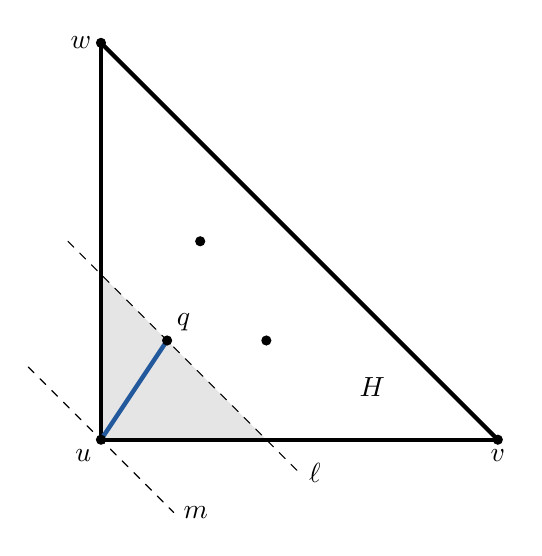
\begin{tikzpicture}[]
\path[fill=black!10] (0.000,0.000) -- (2.100,0.000) -- (0.000,2.100) -- cycle;
\draw[dashed] (-0.924,0.924) -- (0.924,-0.924) node[right] {$m$};
\draw[dashed] (-0.420,2.520) -- (2.520,-0.420) node[right] {$\ell$};
\draw[hull] (0.000,0.000) -- (5.040,0.000);
\draw[hull] (5.040,0.000) -- (0.000,5.040);
\draw[hull] (0.000,5.040) -- (0.000,0.000);
\draw[draw=layerA,line width=1.6pt] (0.000,0.000) -- (0.840,1.260);
\node[vertex] at (0.000,0.000) {};
\node[below left] at (0.000,0.000) {$u$};
\node[vertex] at (5.040,0.000) {};
\node[below] at (5.040,0.000) {$v$};
\node[vertex] at (0.000,5.040) {};
\node[left] at (0.000,5.040) {$w$};
\node[vertex] at (0.840,1.260) {};
\node[above right] at (0.840,1.260) {$q$};
\node[vertex] at (2.100,1.260) {};
\node[vertex] at (1.260,2.520) {};
\node at (3.444,0.672) {$H$};
\end{tikzpicture}

\caption{Lemma~\ref{lem:sweep} for a triangular hull. The line $m$ through $u$ is parallel to $vw$; $q$ is the point nearest to it, and $\ell$ is the parallel through $q$. The shaded strip between $m$ and $\ell$ contains no point of the set, so no segment crosses $uq$ (thick).}\label{fig:sweep}
\end{figure}

\begin{lemma}\label{lem:sweep}
Let $u$ be a hull vertex of $P$ and $m$ a line through $u$ that has all other points of $P$ strictly on one side. If $q$ is a point of $P\setminus\{u\}$ nearest to $m$, then $uq$ is unavoidable.
\end{lemma}

\begin{proof}
Let $\ell$ be the line through $q$ parallel to $m$, and $H$ the closed half-plane bounded by $\ell$ that does not contain $u$. All points of $P$ other than $u$ lie in $H$. Every point of the open segment $uq$ lies strictly between $m$ and $\ell$, hence outside $H$. A segment crossing $uq$ does so at such a point, so it is not contained in $H$; but a segment with both endpoints in $H$ lies in $H$, and a segment with an endpoint at $u$ does not cross $uq$. So no segment crosses $uq$.
\end{proof}

\begin{corollary}\label{cor:lower}
If $P$ has an interior point and its hull has at most four vertices, two triangulations of $P$ share at least six edges. Hence if $|P|\geq5$, two triangulations of $P$ share at least five edges, and if they share exactly five then the hull of $P$ is a pentagon.
\end{corollary}

\begin{proof}
Suppose first that $P$ has an interior point and its hull has at most four vertices. If the hull is a triangle $uvw$, apply Lemma~\ref{lem:sweep} at $u$ with $m$ parallel to $vw$; interior points are closer to $m$ than $v$ and $w$ are, so the resulting segment is interior. Doing the same at $v$ and at $w$ gives three interior unavoidable segments, which are distinct because their hull endpoints differ. With the hull edges that makes six. If the hull is a quadrilateral $uvwx$, one of the triangles $uvx$ and $wvx$ contains an interior point; if it is $uvx$, apply the lemma at $u$ with $m$ parallel to $vx$, and otherwise at $w$. This gives an interior unavoidable segment ending at $u$ or $w$. The diagonal $uw$ gives, in the same way, one ending at $v$ or $x$. With the four hull edges that makes six.

For the second statement, a hull with at least five vertices gives five shared edges on its own. A hull with at most four vertices and $|P|\geq5$ leaves an interior point, and then six edges are shared.
\end{proof}

\section{Nine Points}\label{sec:nine}

Number the points as follows.
\[
\begin{array}{c|ccccccccc}
 i & 1 & 2 & 3 & 4 & 5 & 6 & 7 & 8 & 9\\\hline
 x_i & 33 & 47 & 47 & 29 & 28 & 21 & 23 & 2 & 0\\
 y_i & 47 & 30 & 5 & 20 & 26 & 21 & 29 & 0 & 31
\end{array}
\]
Write $ij$ for the segment from point $i$ to point $j$. The hull is the pentagon $1,2,3,8,9$, with edges $12,23,38,89,91$. Figure~\ref{fig:nine} shows the triangulations
\begin{align*}
A&=\text{hull}\cup\{14,15,16,17,18,24,28,45,48,56,58,67,68,78\},\\
B&=\text{hull}\cup\{25,27,29,34,35,36,37,39,46,47,49,57,69,79\}.
\end{align*}
The two sets of interior edges are disjoint. One checks from the coordinates that no three points are collinear and that no two edges of $A$, or of $B$, cross; the ancillary file \texttt{check\_paper.py} does this in exact arithmetic. Each of $A$ and $B$ then has $19$ pairwise non-crossing edges, and $19=3\cdot9-3-5$ is the number of edges of any triangulation of nine points with five on the hull (Euler's formula), so both are triangulations. Hence $f(9)\leq5$.


\section{Adding a Point}\label{sec:insert}

We want to preserve the property of the nine-point example as points are inserted. Call two triangulations of the same point set \emph{hull-disjoint} if they share only the hull edges.

To add a point without creating a shared edge, it is enough to place it inside a face of $A$ and a face of $B$ that have no vertex in common, and join it to the vertices of each.

\begin{definition}
Let $A$ and $B$ be triangulations of $P$. A face $\alpha$ of $A$ and a face $\beta$ of $B$ form a \emph{good pair} if their interiors intersect and they have no vertex in common.
\end{definition}

For example, in Figure~\ref{fig:nine} the face $156$ of $A$ and the face $479$ of $B$ form a good pair; the point $(24,24)$ lies inside both.

\begin{lemma}[Insertion]\label{lem:insert}
Let $A$ and $B$ be hull-disjoint triangulations of $P$ with a good pair $(\alpha,\beta)$, and let $p\in\inter(\alpha)\cap\inter(\beta)$ lie on no line through two points of $P$. Let $A'$ be $A$ with $p$ joined to the three vertices of $\alpha$, and $B'$ be $B$ with $p$ joined to the three vertices of $\beta$. Then $A'$ and $B'$ are hull-disjoint triangulations of $P\cup\{p\}$.
\end{lemma}

\begin{proof}
As Figure~\ref{fig:insert} illustrates, joining a point inside a face to its three vertices cuts that face into three triangles and leaves everything else unchanged, so $A'$ and $B'$ are triangulations; the hull is the same as before. The old edges of $A'$ and $B'$ are shared only on the hull. The new edges of $A'$ join $p$ to the vertices of $\alpha$, and those of $B'$ join $p$ to the vertices of $\beta$; as $\alpha$ and $\beta$ have no common vertex, no new edge is shared. A suitable $p$ exists because $\inter(\alpha)\cap\inter(\beta)$ is a nonempty open set and only finitely many lines are excluded.
\end{proof}

\begin{figure}[t]
\centering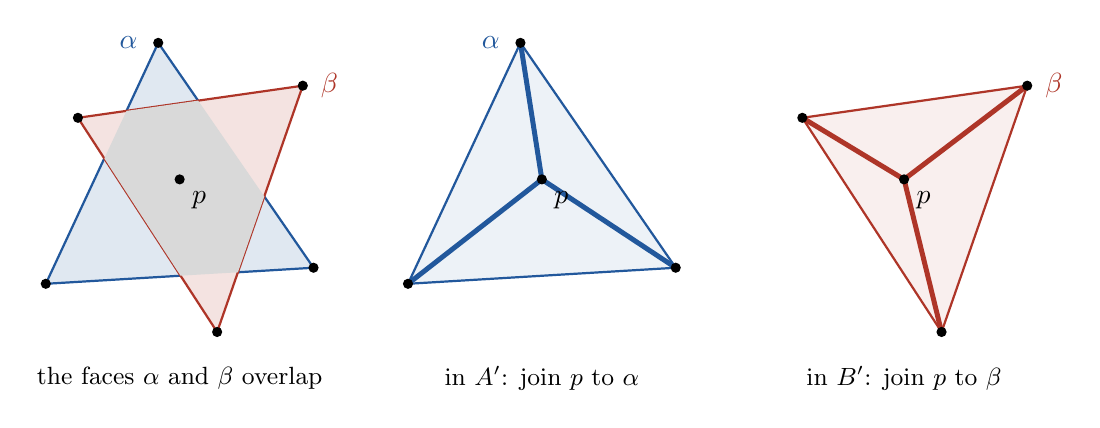
\begin{tikzpicture}[]
\path[fill=layerA!14] (0.000,0.000) -- (3.400,0.204) -- (1.428,3.060) -- cycle;
\path[draw=layerA,line width=.8pt] (0.000,0.000) -- (3.400,0.204) -- (1.428,3.060) -- cycle;
\path[fill=layerB!14] (0.408,2.108) -- (3.264,2.516) -- (2.176,-0.612) -- cycle;
\path[draw=layerB,line width=.8pt] (0.408,2.108) -- (3.264,2.516) -- (2.176,-0.612) -- cycle;
\path[fill=gray!30] (1.711,0.103) -- (2.440,0.146) -- (2.775,1.109) -- (1.935,2.326) -- (1.025,2.196) -- (0.743,1.592) -- cycle;
\node[vertex] at (0.000,0.000) {};
\node[vertex] at (3.400,0.204) {};
\node[vertex] at (1.428,3.060) {};
\node[vertex] at (0.408,2.108) {};
\node[vertex] at (3.264,2.516) {};
\node[vertex] at (2.176,-0.612) {};
\node[vertex] at (1.700,1.326) {};
\node[below right=1pt] at (1.700,1.326) {$p$};
\node[left=4pt,text=layerA] at (1.428,3.060) {$\alpha$};
\node[right=3pt,text=layerB] at (3.264,2.516) {$\beta$};
\node at (1.700,-1.2) {\small the faces $\alpha$ and $\beta$ overlap};
\path[fill=layerA!8] (4.600,0.000) -- (8.000,0.204) -- (6.028,3.060) -- cycle;
\path[draw=layerA,line width=.8pt] (4.600,0.000) -- (8.000,0.204) -- (6.028,3.060) -- cycle;
\draw[draw=layerA,line width=1.8pt] (6.300,1.326) -- (4.600,0.000);
\draw[draw=layerA,line width=1.8pt] (6.300,1.326) -- (8.000,0.204);
\draw[draw=layerA,line width=1.8pt] (6.300,1.326) -- (6.028,3.060);
\node[vertex] at (4.600,0.000) {};
\node[vertex] at (8.000,0.204) {};
\node[vertex] at (6.028,3.060) {};
\node[vertex] at (6.300,1.326) {};
\node[below right=1pt] at (6.300,1.326) {$p$};
\node[left=4pt,text=layerA] at (6.028,3.060) {$\alpha$};
\node at (6.300,-1.2) {\small in $A'$: join $p$ to $\alpha$};
\path[fill=layerB!8] (9.608,2.108) -- (12.464,2.516) -- (11.376,-0.612) -- cycle;
\path[draw=layerB,line width=.8pt] (9.608,2.108) -- (12.464,2.516) -- (11.376,-0.612) -- cycle;
\draw[draw=layerB,line width=1.8pt] (10.900,1.326) -- (9.608,2.108);
\draw[draw=layerB,line width=1.8pt] (10.900,1.326) -- (12.464,2.516);
\draw[draw=layerB,line width=1.8pt] (10.900,1.326) -- (11.376,-0.612);
\node[vertex] at (9.608,2.108) {};
\node[vertex] at (12.464,2.516) {};
\node[vertex] at (11.376,-0.612) {};
\node[vertex] at (10.900,1.326) {};
\node[below right=1pt] at (10.900,1.326) {$p$};
\node[right=3pt,text=layerB] at (12.464,2.516) {$\beta$};
\node at (10.900,-1.2) {\small in $B'$: join $p$ to $\beta$};
\end{tikzpicture}

\caption{Lemma~\ref{lem:insert}. The point $p$ lies in the overlap of $\alpha$ and $\beta$ (shaded). The three thick blue edges are added to $A$ and the three thick red edges to $B$.}\label{fig:insert}
\end{figure}

\section{The Good Pair Returns}\label{sec:regen}

A single insertion is easy; to repeat it, a new good pair is needed after each step. Look again at Figure~\ref{fig:nine}. The side $56$ of the face $156$ of $A$ passes through the faces $357$, $347$, $479$ and $469$ of $B$, in this order from $5$ to $6$. The face $479$ shares no vertex with $156$, so it forms a good pair with $156$ and can receive the next point. The face $347$ contains neither $5$ nor $6$, and it will still lie along the side $56$ after that point is inserted, ready to form the next good pair. Carrying both faces along one side is the whole idea.

\begin{definition}
Let $A$ and $B$ be triangulations of $P$. A face $\alpha=xyz$ of $A$ and two different faces $\beta$ and $\gamma$ of $B$ form a \emph{chain} $(\alpha;\beta,\gamma)$ along the side $xy$ if the open segment $xy$ meets the interiors of both $\beta$ and $\gamma$, $\beta$ has no vertex in common with $\alpha$, and $\gamma$ has neither $x$ nor $y$ as a vertex.
\end{definition}

So $(156;479,347)$ is a chain along $56$.

A chain contains a good pair. Near a point of the open side $xy$ inside $\beta$, the face $\alpha$ contains a half-disc bounded by $xy$, so the interiors of $\alpha$ and $\beta$ meet, and they have no common vertex. So Lemma~\ref{lem:insert} applies to $(\alpha,\beta)$, and the chain survives the insertion.

\begin{lemma}[Regeneration]\label{lem:regen}
Let $A$ and $B$ be hull-disjoint triangulations of $P$ with a chain $(\alpha;\beta,\gamma)$ along the side $xy$ of $\alpha$, and let $A',B'$ be obtained from the good pair $(\alpha,\beta)$ as in Lemma~\ref{lem:insert}. Then some face $\beta'$ of $B'$ inside $\beta$ meets the open segment $xy$, and $(pxy;\gamma,\beta')$ is a chain of $A'$ and $B'$ along $xy$.
\end{lemma}

\begin{proof}
The face $pxy$ of $A'$ has side $xy$. The face $\gamma$ is still a face of $B'$, since only $\beta$ was subdivided, and it still meets the open segment $xy$. Inserting $p$ cuts $\beta$ into three faces along the segments from $p$ to the vertices of $\beta$. Each of these segments meets the line $xy$ at most once, because $p$ is on no line through two points of $P$. The open segment $xy$ meets $\inter(\beta)$ in an open interval, so some point of that interval avoids the three segments and lies inside one of the three faces; call it $\beta'$. It remains to check the vertices. The vertices of $\gamma$ are points of $P$ other than $x$ and $y$, and $p\notin P$, so $\gamma$ has no vertex in common with $pxy$. The vertices of $\beta'$ are $p$ and two vertices of $\beta$, which are neither $x$ nor $y$. Finally $\beta'\subseteq\beta$ is different from $\gamma$.
\end{proof}

\begin{figure}[t]
\centering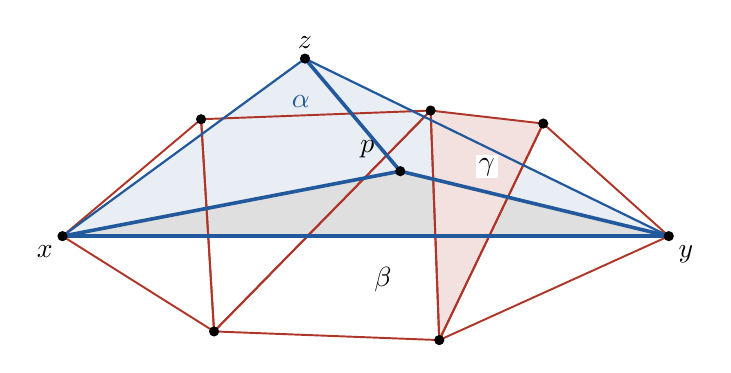
\begin{tikzpicture}[]
\path[fill=layerA!10] (0.000,0.000) -- (7.700,0.000) -- (3.080,2.255) -- cycle;
\path[fill=gray!25] (0.000,0.000) -- (4.290,0.825) -- (7.700,0.000) -- cycle;
\path[fill=layerB!15] (4.785,-1.320) -- (4.675,1.595) -- (6.105,1.430) -- cycle;
\path[draw=layerB,line width=.7pt] (0.000,0.000) -- (1.760,1.485) -- (1.925,-1.210) -- cycle;
\path[draw=layerB,line width=.7pt] (1.925,-1.210) -- (1.760,1.485) -- (4.675,1.595) -- cycle;
\path[draw=layerB,line width=.7pt] (1.925,-1.210) -- (4.675,1.595) -- (4.785,-1.320) -- cycle;
\path[draw=layerB,line width=.7pt] (4.785,-1.320) -- (4.675,1.595) -- (6.105,1.430) -- cycle;
\path[draw=layerB,line width=.7pt] (4.785,-1.320) -- (6.105,1.430) -- (7.700,0.000) -- cycle;
\draw[draw=layerA,line width=.8pt] (0.000,0.000) -- (3.080,2.255);
\draw[draw=layerA,line width=.8pt] (3.080,2.255) -- (7.700,0.000);
\draw[draw=layerA,line width=1.3pt] (4.290,0.825) -- (0.000,0.000);
\draw[draw=layerA,line width=1.3pt] (4.290,0.825) -- (7.700,0.000);
\draw[draw=layerA,line width=1.3pt] (4.290,0.825) -- (3.080,2.255);
\draw[draw=layerA,line width=1.3pt] (0.000,0.000) -- (7.700,0.000);
\node[vertex] at (0.000,0.000) {};
\node[vertex] at (7.700,0.000) {};
\node[vertex] at (3.080,2.255) {};
\node[vertex] at (4.290,0.825) {};
\node[vertex] at (1.760,1.485) {};
\node[vertex] at (1.925,-1.210) {};
\node[vertex] at (4.675,1.595) {};
\node[vertex] at (4.785,-1.320) {};
\node[vertex] at (6.105,1.430) {};
\node[below left] at (0.000,0.000) {$x$};
\node[below right] at (7.700,0.000) {$y$};
\node[above] at (3.080,2.255) {$z$};
\node[inner sep=1pt] at (3.872,1.100) {$p$};
\node[inner sep=1pt,text=layerA] at (3.025,1.705) {$\alpha$};
\node[fill=white,inner sep=1pt] at (4.070,-0.550) {$\beta$};
\node[fill=white,inner sep=1pt] at (5.390,0.880) {$\gamma$};
\end{tikzpicture}

\caption{Lemma~\ref{lem:regen}. The side $xy$ of $\alpha=xyz$ passes through the faces $\beta$ and $\gamma$ of $B$ (red; faces of $B$ away from $xy$ are omitted, and $\beta$ is drawn before it is subdivided). After $p$ is inserted in $\alpha\cap\beta$, the face $pxy$ of $A'$ (grey), the face $\gamma$ (shaded) and a piece of $\beta$ form the next chain.}\label{fig:chain}
\end{figure}

In the example, inserting $p=(24,24)$ in $156\cap479$ gives the chain $(56p;347,\beta')$, where $\beta'$ is the piece $47p$ of $479$. In particular $(56p,347)$ is the next good pair.

\begin{proof}[Proof of Theorem~\ref{thm:main}]
The triangulations of Section~\ref{sec:nine} are hull-disjoint and have the chain $(156;479,347)$. By Lemmas~\ref{lem:insert} and~\ref{lem:regen}, points can be added one at a time, keeping the pentagonal hull, hull-disjoint triangulations and a chain. This gives $f(n)\leq5$ for every $n\geq9$, and Corollary~\ref{cor:lower} gives $f(n)\geq5$.
\end{proof}

At each step the point $p$ can be chosen rational, so for each $n$ the construction yields integer coordinates after clearing denominators.

\section{Why Nine}\label{sec:small}

Aichholzer, Aurenhammer, and Krasser~\cite{AAK} listed all order types of up to ten points in general position. Two point sets have the same order type if some bijection between them preserves the orientation of every triple or reverses all of them, so a set and its mirror image count once; they then have the same crossing pairs of segments and hence the same triangulations. There are $3{,}315$ order types of eight points, $158{,}817$ of nine and $14{,}309{,}547$ of ten.

For a single point set the minimum is a finite computation. Two triangulations of $P$ have $2(3n-3-h)$ edges counted with multiplicity, where $h$ is the number of hull vertices, so they share $2(3n-3-h)-|A\cup B|$ edges; and $A\cup B$ is a set of segments that splits into two non-crossing classes. Conversely, each class of such a split extends to a triangulation. So the minimum number of shared edges is
\[
6n-6-2h-\binom n2+\operatorname{oct}(P),
\]
where $\operatorname{oct}(P)$ is the least number of segments that must be removed from the crossing graph of all $\binom n2$ segments to make it bipartite. In words, $\binom n2-\operatorname{oct}(P)$ is the largest set of segments that splits into two non-crossing classes; this is the largest possible union $A\cup B$, and subtracting it from the $2(3n-3-h)$ edges of $A$ and $B$ leaves the overlap. For a convex pentagon the five hull edges cross nothing and the five diagonals cross in a single $5$-cycle, so $\operatorname{oct}=1$ and the formula gives $30-6-10-10+1=5$: two triangulations of a pentagon can share only the hull.

The crossing graph has one vertex for each segment and an edge for each crossing pair. The search tests whether at most $k$ of its vertices can be deleted to leave a bipartite graph. If an odd cycle remains, every successful deletion set must contain a vertex of that cycle; branching over all its vertices is therefore exhaustive. A branch stops when the remaining graph is bipartite or its deletion budget is exhausted. Vertex-disjoint odd cycles give a lower bound on the deletions needed and allow branches to be pruned. All orientation tests and graph operations use exact integer arithmetic.

For the computer-dependent part of Theorem~\ref{thm:hull}, the database has $3$, $22$ and $570$ pentagonal-hull order types on six, seven and eight points respectively. None permits only five shared edges. The ancillary files give commands, expected counts and hashes of the input files, so this small negative result can be reproduced separately from the larger searches.

Evaluating the formula for every order type gives, for point sets in general position,
\[
\begin{array}{c|ccccccc}
 n & 4 & 5 & 6 & 7 & 8 & 9 & 10\\\hline
 \min|A\cap B| & 4 & 5 & 6 & 6 & 6 & 5 & 5
\end{array}
\]
So the minimum rises to six and returns to five at $n=9$. Exactly seven order types of nine points and $734$ of ten attain five, all with pentagonal hulls; the set of Section~\ref{sec:nine} is one of the seven. For a triangular hull the minimum is seven when $n=9$ and when $n=10$, which means that the largest doubly linear graphs on nine or ten points in general position have $6n-19$ edges. The ancillary files contain the search program, its output, and an independent check of the seven nine-point sets.

\section{Other Hulls}\label{sec:hulls}

To start the construction of Section~\ref{sec:regen} with another hull size, we need hull-disjoint triangulations with a chain. Convex polygons provide them.

\begin{lemma}[Convex seed]\label{lem:convex}
Let $v_1,\dots,v_h$ be the vertices of a convex polygon in order around it, with $h\geq6$, and let
\begin{align*}
A&=\text{hull}\cup\{v_1v_3,\,v_3v_5,\,v_1v_5\}\cup\{v_5v_k: 7\leq k\leq h\},\\
B&=\text{hull}\cup\{v_2v_4,\,v_4v_6,\,v_2v_6\}\cup\{v_2v_k: 7\leq k\leq h\}.
\end{align*}
Then $A$ and $B$ are hull-disjoint triangulations of $\{v_1,\dots,v_h\}$. If $h\geq7$, the face $v_1v_3v_5$ of $A$ and the faces $v_2v_4v_6$ and $v_2v_6v_7$ of $B$ form a chain along $v_1v_3$.
\end{lemma}

\begin{figure}[t]
\centering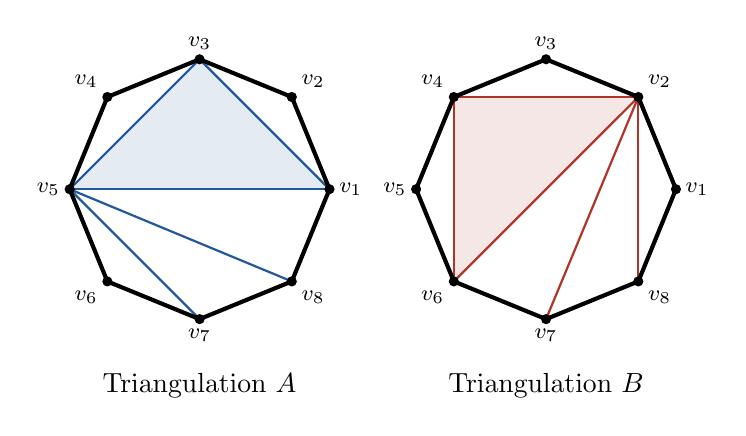
\begin{tikzpicture}[]
\path[fill=layerA!12] (1.650,0.000) -- (0.000,1.650) -- (-1.650,0.000) -- cycle;
\draw[draw=layerA,line width=.8pt] (1.650,0.000) -- (0.000,1.650);
\draw[draw=layerA,line width=.8pt] (1.650,0.000) -- (-1.650,0.000);
\draw[draw=layerA,line width=.8pt] (0.000,1.650) -- (-1.650,0.000);
\draw[draw=layerA,line width=.8pt] (-1.650,0.000) -- (0.000,-1.650);
\draw[draw=layerA,line width=.8pt] (-1.650,0.000) -- (1.171,-1.171);
\draw[hull] (1.650,0.000) -- (1.171,1.171);
\draw[hull] (1.650,0.000) -- (1.171,-1.171);
\draw[hull] (1.171,1.171) -- (0.000,1.650);
\draw[hull] (0.000,1.650) -- (-1.171,1.171);
\draw[hull] (-1.171,1.171) -- (-1.650,0.000);
\draw[hull] (-1.650,0.000) -- (-1.171,-1.171);
\draw[hull] (-1.171,-1.171) -- (0.000,-1.650);
\draw[hull] (0.000,-1.650) -- (1.171,-1.171);
\node[vertex] at (1.650,0.000) {};
\node[right,font=\footnotesize] at (1.650,0.000) {$v_1$};
\node[vertex] at (1.171,1.171) {};
\node[above right,font=\footnotesize] at (1.171,1.171) {$v_2$};
\node[vertex] at (0.000,1.650) {};
\node[above,font=\footnotesize] at (0.000,1.650) {$v_3$};
\node[vertex] at (-1.171,1.171) {};
\node[above left,font=\footnotesize] at (-1.171,1.171) {$v_4$};
\node[vertex] at (-1.650,0.000) {};
\node[left,font=\footnotesize] at (-1.650,0.000) {$v_5$};
\node[vertex] at (-1.171,-1.171) {};
\node[below left,font=\footnotesize] at (-1.171,-1.171) {$v_6$};
\node[vertex] at (0.000,-1.650) {};
\node[below,font=\footnotesize] at (0.000,-1.650) {$v_7$};
\node[vertex] at (1.171,-1.171) {};
\node[below right,font=\footnotesize] at (1.171,-1.171) {$v_8$};
\node at (0.000,-2.5) {Triangulation $A$};
\path[fill=layerB!12] (5.572,1.171) -- (3.229,1.171) -- (3.229,-1.171) -- cycle;
\draw[draw=layerB,line width=.8pt] (5.572,1.171) -- (3.229,1.171);
\draw[draw=layerB,line width=.8pt] (5.572,1.171) -- (3.229,-1.171);
\draw[draw=layerB,line width=.8pt] (5.572,1.171) -- (4.400,-1.650);
\draw[draw=layerB,line width=.8pt] (5.572,1.171) -- (5.572,-1.171);
\draw[draw=layerB,line width=.8pt] (3.229,1.171) -- (3.229,-1.171);
\draw[hull] (6.050,0.000) -- (5.572,1.171);
\draw[hull] (6.050,0.000) -- (5.572,-1.171);
\draw[hull] (5.572,1.171) -- (4.400,1.650);
\draw[hull] (4.400,1.650) -- (3.229,1.171);
\draw[hull] (3.229,1.171) -- (2.750,0.000);
\draw[hull] (2.750,0.000) -- (3.229,-1.171);
\draw[hull] (3.229,-1.171) -- (4.400,-1.650);
\draw[hull] (4.400,-1.650) -- (5.572,-1.171);
\node[vertex] at (6.050,0.000) {};
\node[right,font=\footnotesize] at (6.050,0.000) {$v_1$};
\node[vertex] at (5.572,1.171) {};
\node[above right,font=\footnotesize] at (5.572,1.171) {$v_2$};
\node[vertex] at (4.400,1.650) {};
\node[above,font=\footnotesize] at (4.400,1.650) {$v_3$};
\node[vertex] at (3.229,1.171) {};
\node[above left,font=\footnotesize] at (3.229,1.171) {$v_4$};
\node[vertex] at (2.750,0.000) {};
\node[left,font=\footnotesize] at (2.750,0.000) {$v_5$};
\node[vertex] at (3.229,-1.171) {};
\node[below left,font=\footnotesize] at (3.229,-1.171) {$v_6$};
\node[vertex] at (4.400,-1.650) {};
\node[below,font=\footnotesize] at (4.400,-1.650) {$v_7$};
\node[vertex] at (5.572,-1.171) {};
\node[below right,font=\footnotesize] at (5.572,-1.171) {$v_8$};
\node at (4.400,-2.5) {Triangulation $B$};
\end{tikzpicture}

\caption{Lemma~\ref{lem:convex} for $h=8$. The side $v_1v_3$ of the shaded face $v_1v_3v_5$ of $A$ passes through the faces $v_2v_4v_6$ (shaded) and $v_2v_6v_7$ of $B$. For $h=6$ the fans are empty.}\label{fig:convex}
\end{figure}

\begin{proof}
The triangle $v_1v_3v_5$ cuts the polygon into itself, the ears $v_1v_2v_3$ and $v_3v_4v_5$, and the convex polygon $v_5v_6\cdots v_hv_1$, which the segments $v_5v_k$ triangulate as a fan from $v_5$. So $A$ is a triangulation. The same argument, with every index increased by one, shows that $B$ is one: its pieces are $v_2v_4v_6$, the ears $v_2v_3v_4$ and $v_4v_5v_6$, and the polygon $v_6\cdots v_hv_1v_2$ fanned from $v_2$. Every interior edge of $B$ has an endpoint among $v_2,v_4,v_6$, and no interior edge of $A$ does, so $A$ and $B$ share only the hull. Now let $h\geq7$. The segment $v_1v_3$ separates $v_2$ from the other vertices, so it crosses every segment from $v_2$ to another vertex except the two hull edges at $v_2$. In particular it crosses the sides $v_2v_4$ and $v_2v_6$ of $v_2v_4v_6$, and the sides $v_2v_6$ and $v_2v_7$ of $v_2v_6v_7$, and so meets the interiors of both faces. The face $v_2v_4v_6$ has no vertex in common with $v_1v_3v_5$, and $v_2v_6v_7$ contains neither $v_1$ nor $v_3$.
\end{proof}

For $h=6$ these triangulations have no chain. Every side of a face of $A$ that is not a hull edge is a side of $v_1v_3v_5$. The side $v_1v_3$ passes through only three faces of $B$, namely $v_6v_1v_2$, $v_2v_4v_6$ and $v_2v_3v_4$, and the outer two contain $v_1$ or $v_3$; by symmetry the same holds for $v_3v_5$ and $v_5v_1$. So the hexagonal case needs a different start, and seven points suffice.

Number the points as follows.
\[
\begin{array}{c|ccccccc}
 i & 1 & 2 & 3 & 4 & 5 & 6 & 7\\\hline
 x_i & 1 & 0 & 1 & 4 & 5 & 6 & 2\\
 y_i & 2 & 0 & 0 & 1 & 2 & 6 & 1
\end{array}
\]
The hull is the hexagon $1,2,3,4,5,6$, and point $7$ lies inside it. Figure~\ref{fig:seven} shows the triangulations
\begin{align*}
A&=\text{hull}\cup\{13,14,15,17,37,47\},\\
B&=\text{hull}\cup\{24,25,26,27,57,67\}.
\end{align*}
As in Section~\ref{sec:nine}, one checks from the coordinates that no three points are collinear and that no two edges of $A$, or of $B$, cross. Each has $12=3\cdot7-3-6$ edges, so both are triangulations, and their interior edges are disjoint. The side $13$ of the face $137$ of $A$ passes through the faces $245$ and $267$ of $B$ (the point $(6/5,2/5)$ lies inside $137$ and $245$). The face $245$ shares no vertex with $137$, and $267$ contains neither $1$ nor $3$, so $(137;245,267)$ is a chain along $13$.

\begin{figure}[t]
\centering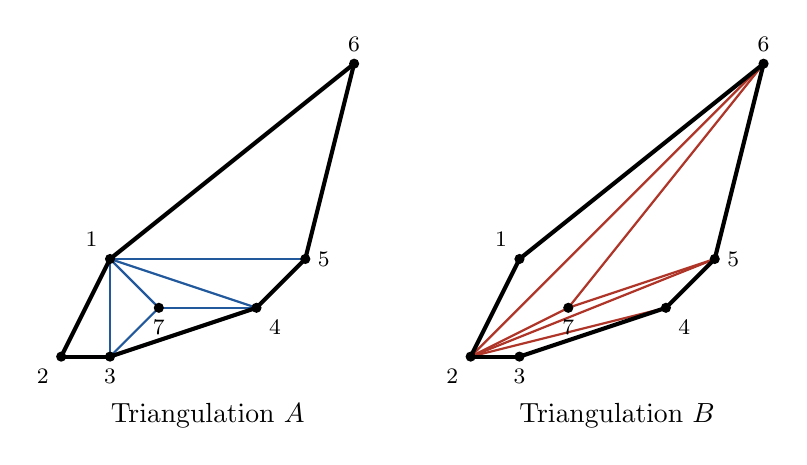
\begin{tikzpicture}[]
\draw[draw=layerA,line width=.8pt] (0.620,1.240) -- (0.620,0.000);
\draw[draw=layerA,line width=.8pt] (0.620,1.240) -- (2.480,0.620);
\draw[draw=layerA,line width=.8pt] (0.620,1.240) -- (3.100,1.240);
\draw[draw=layerA,line width=.8pt] (0.620,1.240) -- (1.240,0.620);
\draw[draw=layerA,line width=.8pt] (0.620,0.000) -- (1.240,0.620);
\draw[draw=layerA,line width=.8pt] (2.480,0.620) -- (1.240,0.620);
\draw[hull] (0.620,1.240) -- (0.000,0.000);
\draw[hull] (0.620,1.240) -- (3.720,3.720);
\draw[hull] (0.000,0.000) -- (0.620,0.000);
\draw[hull] (0.620,0.000) -- (2.480,0.620);
\draw[hull] (2.480,0.620) -- (3.100,1.240);
\draw[hull] (3.100,1.240) -- (3.720,3.720);
\node[vertex] at (0.620,1.240) {};
\node[above left=1pt,font=\footnotesize] at (0.620,1.240) {$1$};
\node[vertex] at (0.000,0.000) {};
\node[below left=1pt,font=\footnotesize] at (0.000,0.000) {$2$};
\node[vertex] at (0.620,0.000) {};
\node[below=1pt,font=\footnotesize] at (0.620,0.000) {$3$};
\node[vertex] at (2.480,0.620) {};
\node[below right=1pt,font=\footnotesize] at (2.480,0.620) {$4$};
\node[vertex] at (3.100,1.240) {};
\node[right=1pt,font=\footnotesize] at (3.100,1.240) {$5$};
\node[vertex] at (3.720,3.720) {};
\node[above=1pt,font=\footnotesize] at (3.720,3.720) {$6$};
\node[vertex] at (1.240,0.620) {};
\node[below=1pt,font=\footnotesize] at (1.240,0.620) {$7$};
\node at (1.860,-0.75) {Triangulation $A$};
\draw[draw=layerB,line width=.8pt] (5.200,0.000) -- (7.680,0.620);
\draw[draw=layerB,line width=.8pt] (5.200,0.000) -- (8.300,1.240);
\draw[draw=layerB,line width=.8pt] (5.200,0.000) -- (8.920,3.720);
\draw[draw=layerB,line width=.8pt] (5.200,0.000) -- (6.440,0.620);
\draw[draw=layerB,line width=.8pt] (8.300,1.240) -- (6.440,0.620);
\draw[draw=layerB,line width=.8pt] (8.920,3.720) -- (6.440,0.620);
\draw[hull] (5.820,1.240) -- (5.200,0.000);
\draw[hull] (5.820,1.240) -- (8.920,3.720);
\draw[hull] (5.200,0.000) -- (5.820,0.000);
\draw[hull] (5.820,0.000) -- (7.680,0.620);
\draw[hull] (7.680,0.620) -- (8.300,1.240);
\draw[hull] (8.300,1.240) -- (8.920,3.720);
\node[vertex] at (5.820,1.240) {};
\node[above left=1pt,font=\footnotesize] at (5.820,1.240) {$1$};
\node[vertex] at (5.200,0.000) {};
\node[below left=1pt,font=\footnotesize] at (5.200,0.000) {$2$};
\node[vertex] at (5.820,0.000) {};
\node[below=1pt,font=\footnotesize] at (5.820,0.000) {$3$};
\node[vertex] at (7.680,0.620) {};
\node[below right=1pt,font=\footnotesize] at (7.680,0.620) {$4$};
\node[vertex] at (8.300,1.240) {};
\node[right=1pt,font=\footnotesize] at (8.300,1.240) {$5$};
\node[vertex] at (8.920,3.720) {};
\node[above=1pt,font=\footnotesize] at (8.920,3.720) {$6$};
\node[vertex] at (6.440,0.620) {};
\node[below=1pt,font=\footnotesize] at (6.440,0.620) {$7$};
\node at (7.060,-0.75) {Triangulation $B$};
\end{tikzpicture}

\caption{Two triangulations of seven points with a hexagonal hull, sharing only the six hull edges (black).}\label{fig:seven}
\end{figure}

\begin{proof}[Proof of Theorem~\ref{thm:hull}]
Suppose first that $n=h$, so the points are in convex position. For $h=3$ the only triangulation has no interior edge. For $h=4$ the two diagonals give two triangulations sharing only the hull, and for $h=5$ so do the fans $\{v_1v_3,v_1v_4\}$ and $\{v_2v_4,v_2v_5\}$. For $h\geq6$, Lemma~\ref{lem:convex} applies.

Now let $n>h$, so that $P$ has an interior point. If $h\leq4$, Corollary~\ref{cor:lower} gives at least six shared edges, which is more than $h$. If $h=5$, the table in Section~\ref{sec:small} shows that two triangulations of six, seven or eight points share at least six edges, and Theorem~\ref{thm:main} covers every $n\geq9$. If $h\geq7$, start from the chain of Lemma~\ref{lem:convex}. Lemmas~\ref{lem:insert} and~\ref{lem:regen} add interior points one at a time, keeping the hull, hull-disjoint triangulations and a chain, and every $n>h$ is reached. If $h=6$, start in the same way from the seven points above.
\end{proof}

A longer argument, included in the Lean formalisation described in the acknowledgements, shows that once $|P|\geq7$ every good pair of hull-disjoint triangulations is followed by another after an insertion, with no chain needed; the hexagon of the convex seed is where this fails. The part of the proof for a pentagonal hull with six to eight points is the only one that rests on the computer search; a proof by hand would be welcome. The enumeration agrees with Theorem~\ref{thm:hull} throughout its range: for every $n\leq9$ and every $h$, some order type with $n$ points and $h$ hull vertices has two triangulations sharing only the hull exactly when the theorem says so.

We end with two further questions. Is the minimum for a triangular hull equal to seven for every $n\geq9$? And can a set of six, seven, or eight points with collinear triples, which the enumeration does not include, have two triangulations sharing only five edges?

\section*{Acknowledgements}
The problem and its first bounds come from the MathOverflow discussion~\cite{MO}, in particular the contributions of Tony Huynh, G\"unter Rote, and Jukka Kohonen. Claude Opus~5.5 and Claude Fable~5.1 (Anthropic) were used to search for examples, to write and run the verification code, to develop and check the proofs, and to draft the manuscript. The author is responsible for the content. The ancillary files of this article contain an exact checker for the examples and small claims, including those of Section~\ref{sec:hulls}, the enumeration code, and coordinates and both triangulations for $9\leq n\leq17$. Theorems~\ref{thm:main} and~\ref{thm:hull} and the lemmas they use have also been formalised in the Lean~4 proof assistant, with Lemma~\ref{lem:convex} checked for points on a parabola, which is the case the proof of Theorem~\ref{thm:hull} uses. The formalisation takes the computer search of Section~\ref{sec:small} as a stated hypothesis for a pentagonal hull with six to eight points, and the supplementary archive includes the Lean sources, pinned dependency versions, build instructions and a driver that prints the theorem statements and their axiom dependencies. OpenAI ChatGPT assisted with the subsequent exposition and reproducibility revision.
\ifanon\else
The certificates are also available at~\cite{repo}.
\fi

\begin{thebibliography}{9}
\bibitem{AAK}
O.~Aichholzer, F.~Aurenhammer, and H.~Krasser, Enumerating order types for small point sets with applications, \emph{Order} \textbf{19} (2002), no.~3, 265--281. \href{https://doi.org/10.1023/A:1021231927255}{doi:10.1023/A:1021231927255}.
\bibitem{DGM}
S.~Durocher, E.~Gethner, and D.~Mondal, Thickness and colorability of geometric graphs, \emph{Comput. Geom.} \textbf{56} (2016), 1--18. \href{https://doi.org/10.1016/j.comgeo.2016.03.003}{doi:10.1016/j.comgeo.2016.03.003}.
\bibitem{GHK}
A.~Garc\'{\i}a, F.~Hurtado, M.~Korman, I.~Matos, M.~Saumell, R.~I.~Silveira, J.~Tejel, and C.~D.~T\'oth, Geometric biplane graphs~I: maximal graphs, \emph{Graphs Combin.} \textbf{31} (2015), no.~2, 407--425. \href{https://doi.org/10.1007/s00373-015-1546-1}{doi:10.1007/s00373-015-1546-1}.
\bibitem{HSV}
J.~P.~Hutchinson, T.~C.~Shermer, and A.~Vince, On representations of some thickness-two graphs, \emph{Comput. Geom.} \textbf{13} (1999), no.~3, 161--171. \href{https://doi.org/10.1016/S0925-7721(99)00018-8}{doi:10.1016/S0925-7721(99)00018-8}.
\bibitem{MO}
Till, \emph{Minimum number of common edges of triangulations}, MathOverflow question 454425 (12 September 2023), with answers and comments, \url{https://mathoverflow.net/q/454425}.
\bibitem{MOAnswer}
V.~Jandhyala, answer to MathOverflow question 454425, 30 September 2026, \url{https://mathoverflow.net/a/515648}.
\ifanon\else
\bibitem{repo}
\url{https://github.com/jvvk/triangulations-sharing-five-edges}.
\fi
\end{thebibliography}

\end{document}
